% !TEX program = lualatex
\documentclass[10pt, leqno]{ltjsarticle}
% \documentclass[10pt]{ltjsarticle} % 日本語をそのまま扱えるクラス
% \usepackage[margin=28mm]{geometry}
\usepackage{amsmath,amssymb,mathtools}
\usepackage{amsthm}
\usepackage{tikz}
\usetikzlibrary{arrows.meta,positioning,calc}

\usepackage[
  top=15mm,     % 上余白
  bottom=15mm,  % 下余白
  left=10mm,    % 左余白
  right=10mm,    % 右余白
  landscape,
  margin=10mm
]{geometry}
% \usepackage[landscape,margin=20mm]{geometry} % 余白はお好みで
\usepackage{paracol}
\columnratio{0.5,0.5}             % 左右を 1:1 に
\setlength{\columnseprule}{0.4pt} % 真ん中の縦線

% ---- 記号・マクロ ----
\newcommand{\xto}{\mathrel{\xrightarrow{}}}
\newcommand{\into}{\hookrightarrow}
\newcommand{\epi}{\twoheadrightarrow}
\newcommand{\pto}{\rightrightarrows}
\newcommand{\cls}[1]{\bigl(#1\bigr)}
\newcommand{\redjoin}{\wedge}
\newcommand{\shrink}{\phi}
\newcommand{\Ex}{E}        % suspension functor E
\newcommand{\Ox}{\Omega}   % loop functor Omega
\newcommand{\id}{\mathrm{id}}
% --- Toda bracket helpers ---
\newcommand{\toda}[1]{\{\,#1\,\}}              % {a,b,c}
\newcommand{\todai}[2][]{\{\,#2\,\}_{#1}}      % {a,b,c}_i   (#1 は添字, 空なら無し) 
\newcommand{\todas}[1]{\langle\,#1\,\rangle}
\newcommand{\gen}[1]{\{\,#1\,\}}       % ⟨generator⟩ 表記を { } で統一
\newcommand{\Ker}{\operatorname{Ker}}
\newcommand{\im}{\operatorname{Im}}
\newcommand{\hs}[2]{\bigl[#1,#2\bigr]}   % 一般のホモトピー集合
\newcommand{\pis}[2]{\pi_{#1}(#2)}       % 左が球面のときのホモトピー群
\newcommand{\pit}[2]{\pi_{#1}^{#2}}
\newcommand{\ext}[1]{\overline{#1}}     % extension
\newcommand{\coext}[1]{\widetilde{#1}}  % coextension
\newcommand{\z}{\mathbb{Z}}
\newcommand{\sq}[1]{Sq^{#1}}
\newcommand{\map}{\operatorname{Map}}

% ---- theorem-like environments ----
\numberwithin{equation}{section}
\theoremstyle{plain}
\newtheorem{theorem}{Theorem}[section]
\newtheorem{lemma}[theorem]{Lemma}
\newtheorem{proposition}[theorem]{Proposition}
\newtheorem{corollary}[theorem]{Corollary}
\theoremstyle{definition}
\newtheorem{definition}[theorem]{Definition}
\newtheorem{example}[theorem]{Example}
\newtheorem{notation}[theorem]{Notation}
\newtheorem{assumption}[theorem]{Assumption}
\theoremstyle{remark}
\newtheorem{remark}[]{Remark}

% \title{PART 1 \quad CHAPTER I\\[2mm] General Composition and Secondary Composition}
% \author{}
% \date{}

\begin{document}

\setcounter{section}{2}
\section{Reduced Join and Stable Groups}

\begin{paracol}{2}

$\alpha\in\pi_{p+k}(S^p)$, $\beta\in\pi_{q+h}(S^q)$ に対し, 
reduced join
\[
\alpha \wedge \beta\ \in\ \pi_{p+q+k+h}(S^{p+q})
\]
を考える. 

\begin{proposition}[Barratt-Hilton \cite{BarrattHilton1953}]\label{prop:3.1}
% Prop3.1
\[
\alpha \wedge \beta
= (-1)^{(p+k)h} E^{q}\alpha \circ E^{p+k}\beta
= (-1)^{ph} E^{p}\beta \circ E^{q+h}\alpha .
\]
\end{proposition}

\noindent
\textbf{Proof.}\
$\alpha \wedge \iota_n = E^{n}\alpha$ は既知である. \\
$\sigma_{r,s}:S^{r+s}\to S^{r+s}$ を,
\(\sigma_{r,s}(\phi_{r,s}(x,y)) = \phi_{s,r}(y,x)\) で定める.\\
\(\sigma_{r,s}\) は, 
$\deg(\sigma_{r,s})=(-1)^{rs}$ の同相写像である. 
次の関係式が成り立つ.
\[
\iota_n \wedge \alpha
= [\sigma_{p,n}] \circ (\alpha \wedge \iota_n) \circ [\sigma_{n,p+k}]
= (-1)^{pn}\iota_{p+n}\circ E^n\alpha\circ (-1)^{(p+k)n}\iota_{p+k+n}.
\]
(2.1) から,
\(
\iota_n \wedge \alpha = (-1)^{kn} E^{n}\alpha
\)
を得る. さらに, (1.5) から,
\[
\begin{align*}
\alpha \wedge \beta
& = (\alpha\circ\iota_{p+k}) \wedge (\iota_q\circ\beta)
= (\alpha \wedge \iota_q) \circ (\iota_{p+k} \wedge \beta)\\
& = (-1)^{(p+k)h} E^{q}\alpha \circ E^{p+k}\beta,
\end{align*}
\]
\[
\begin{align*}
\alpha \wedge \beta
& = (\iota_p\circ \alpha) \wedge (\beta\circ \iota_{q+h})
= (\iota_p\wedge \beta) \circ (\alpha\wedge\iota_{q+h})\\
& = (-1)^{ph} E^{p}\beta\circ E^{q+h}\alpha.
\end{align*}
\]
\qed

差
\(
E^{q-1}\alpha \circ E^{p+k-1}\beta
 - (-1)^{kh} E^{p-1}\beta \circ E^{q+h-1}\alpha
\)
は, 懸垂準同型 $E$ の下で消える. \\
したがって, これは (2.11) の完全列における
$\Delta$ の像となっている.\\ 
この元に対する次の結果は, \cite{Toda1957} Th.(4.6) に示されている. 

\begin{proposition}\label{prop:3.2}
% Prop3.2.\
$\alpha\in\pi_{p+k}(S^p)$, $\beta\in\pi_{q+h}(S^q)$ とし, \\
\(k\le \min\{\,p+q-3,\ 2p-4\,\},\
h\le \min\{\,p+q-3,\ 2q-4\,\}\)
を仮定する. このとき,
\[
\begin{align*}
& E^{q-1}\alpha \circ E^{p+k-1}\beta
 - (-1)^{kh}E^{p-1}\beta\circ E^{q+h-1}\alpha  \\
& = [\iota_{p+q-1}, \iota_{p+q-1}]\circ 
E^{2q-2}H(\alpha)\circ E^{p+k-1}H(\beta) .\\
& 2([\iota_{p+q-1}, \iota_{p+q-1}]\circ 
E^{2q-2}H(\alpha)\circ E^{p+k-1}H(\beta)) = 0.
\end{align*}
\]
\end{proposition}
(最近, この公式は, \(k\) と \(h\) の制限のないものが作られた \cite{Barratt1961})

\switchcolumn

\noindent
\textbf{
\cite{BarrattHilton1953}
M.~G.~Barratt and P.~J.~Hilton,}
\newblock On join operations of homotopy groups,
\newblock Proc. London Math. Soc., {\bf 3} (1953), 430--445.

\noindent
\textbf{
\cite{Toda1957}
H.~Toda,}
\newblock Reduced join and Whitehead product,
\newblock Jour. of Inst. Poly. Osaka City Univ., {\bf 8} (1957), 15--30.

\noindent
\textbf{
\cite{Barratt1961}
M.~G.~Barratt,}
\newblock Note on a formula due to Toda,
\newblock Jour. London Math. Soc., {\bf 36} (1961), 95--96.

\end{paracol}

\begin{paracol}{2}

Prop2.5 により, 次が成り立つ. 
\[
[\iota_{p+q-1}, \iota_{p+q-1}]\circ E^{2q-2}H(\alpha)\circ E^{p+k-1}H(\beta)
\]
\[
\in \Delta(E^{2q}H(\alpha)\circ E^{p+k+1}H(\beta))
\subset\pi_{p+q+k+h-1}(S^{p+q-1}).
\]
Prop3.2 の仮定から, \(p+q+k+h\le 3(p+q-1)-3\) である. \\
このとき, \(\Delta\) は1つの値を取る. よって, 次の Cor を得る. 

\begin{corollary}\label{cor:3.3}
% Cor3.3
Prop$3.2$ と同じ仮定のもとで,
\[
E^{q-1}\alpha\circ E^{p+k-1}\beta
 - (-1)^{kh} E^{p-1}\beta\circ E^{q+h-1}\alpha
 = \Delta(E^{2q}H(\alpha)\circ E^{p+k-1}H(\beta)).
\]
\end{corollary}

reduced join を用いると, Toda bracket についてのいくつかの関係が得られる. 

\begin{proposition}[\cite{Toda1959} Prop4.6]\label{prop:3.4}
% Prop3.4\
\begin{enumerate}
  % \itemsep4pt
\item[\textup{i)}]
$\alpha\in\pi_{p+h}(S^p)$, 
$\beta\in\pi_{q+k}(S^q)$, 
$\gamma\in\pi_{r+\ell}(S^r)$ が,\\
\(\alpha \wedge \beta = 0,\ \beta \wedge \gamma = 0\)
を満たすとする. \\
このとき, 次の $2$ つの Toda bracket は, 共通元を持つ.
\[
\toda{E^{q+r}\alpha,\ E^{p+h+r}\beta,\ E^{p+h+q+k}\gamma}, 
\]
\[
(-1)^{hk+k\ell+\ell h+1}\,\toda{E^{p+q}\gamma,\ E^{p+r+\ell}\beta,\ 
E^{q+k+r+\ell}\alpha}.
\]
\item[\textup{ii)}]
さらに, $\alpha \wedge \gamma=0$ も満たすとき, 次の和は \(0\) を含む. 
\[
\begin{aligned}
&\ (-1)^{h\ell} \toda{E^{q+r}\alpha,\ E^{p+h+r}\beta,\ E^{p+h+q+k}\gamma}\\
&+\;(-1)^{kh}\toda{E^{p+r}\beta,\ E^{p+q+k}\gamma,\ E^{q+k+r+\ell}\alpha}\\
&+\;(-1)^{\ell k}\toda{E^{p+q}\gamma,\ E^{q+r+\ell}\alpha,\ E^{p+h+r+\ell}\beta} .
\end{aligned}
\]
\end{enumerate}
\end{proposition}

\noindent
\textbf{Proof.}\ 
$[a]=\alpha,[b]=\beta,[c]=\gamma$ とし, 
$a \wedge b, b \wedge c$ の null-homotopy を,
$A_t$, $B_t$ とする. \\
また, $S^n$ の恒等写像を $i_n$ と記す. \\
$H,\ H':S^{s+1}\to S^{p+q+r}$ ($s=p+h+q+k+r+\ell$) を, 次で与える：
\[
H(d_s(x,t))=
\begin{cases}
\bigl(a \wedge i_{q+r}\bigr)\bigl(1_{p+h} \wedge B_{2t-1}\bigr)(x), & \tfrac12\le t\le1,\\[2pt]
\bigl(A_{1-2t} \wedge 1_r\bigr)\bigl(1_{p+h+q+k} \wedge c\bigr)(x), & 0\le t\le\tfrac12,\\[2pt]
\end{cases}
\]
\[
H'(d_s(x,t))=
\begin{cases}
\bigl(1_{p+q} \wedge c\bigr)\bigl(A_{2t-1} \wedge 1_{r+\ell}\bigr)(x), & \tfrac12\le t\le1,\\[2pt]
\bigl(1_p \wedge B_{1-2t}\bigr)\bigl(a \wedge 1_{q+k+r+\ell}\bigr)(x), & 0\le t\le\tfrac12.
\end{cases}
\]
このとき, $H$ は次の元を表す. 
\[
\begin{align*}
& \toda{\alpha \wedge \iota_{q+r},
\iota_{p+h} \wedge \beta, 
\iota_{p+h+q+k} \wedge \gamma}\\
& = \toda{E^{q+r}\alpha, 
(-1)^{(p+h)k}E^{p+h+r}\beta, 
(-1)^{(p+h+q+k)\ell}E^{p+h+q+k}\gamma}\\
& =(-1)^\varepsilon\toda{E^{q+r}\alpha, 
E^{p+h+r}\beta, 
E^{p+h+q+k}\gamma}.\\
& \text{ここで, } \varepsilon = 
(p+h)k + (p+h+q+k)\ell = 
(p+q)\ell + pk + hk + k\ell + \ell h .
\end{align*}
\]

\switchcolumn

\noindent
\textbf{Prop2.5.}\
$\alpha\in\pi_{i+1}(S^{2m+1}), \ \beta\in \pi_{j-1}(S^{i-1})$ 対して, 
\(
\Delta\alpha\ \circ\ \beta\ \subset\ \Delta(\alpha\circ E^2\beta).
\)\\
特に, 任意の $\gamma$ に対し,
\(
\Delta(E^2\gamma)\ \ni\ \pm\,[\,\iota_m,\ \iota_m\,]\circ\gamma
\)
が成り立つ. \\
ここで $[\, ,\,]$ は Whitehead product を表す. \\
上の「$\subset$」および「$\ni$」は, $m$ が奇数, 
あるいは $j<3m-1$, \\
または, 関係する元が \(2\)-primary 成分にあるときには, 
等号「$=$」に置き換えられる. 

\noindent
\textbf{Prop3.2.}\
$\alpha\in\pi_{p+k}(S^p)$, $\beta\in\pi_{q+h}(S^q)$ とし, \\
\(k\le \min\{\,p+q-3,\ 2p-4\,\},\
h\le \min\{\,p+q-3,\ 2q-4\,\}\)
を仮定する. このとき,\\
\(
E^{q-1}\alpha \circ E^{p+k-1}\beta
 - (-1)^{kh}E^{p-1}\beta\circ E^{q+h-1}\alpha 
\)\\
\(
= [\iota_{p+q-1}, \iota_{p+q-1}]\circ 
E^{2q-2}H(\alpha)\circ E^{p+k-1}H(\beta) .
\)\\
\(
2([\iota_{p+q-1}, \iota_{p+q-1}]\circ 
E^{2q-2}H(\alpha)\circ E^{p+k-1}H(\beta)) = 0.
\)

\noindent
\textbf{
\cite{Toda1959}
H.~Toda,}
\newblock $p$-primary components of homotopy groups IV. Compositions and toric constructions,
\newblock Memoirs Univ. of Kyoto, {\bf 32} (1959), 297--332.



\end{paracol}

\begin{paracol}{2}

\noindent
\(H'\) は次の元を表す.
\[
\begin{align*}
& \toda{\iota_{p+q}\wedge \gamma, 
\iota_p\wedge \beta\wedge \iota_{r+\ell}, 
\alpha\wedge\iota_{q+k+r+\ell}}\\
& =\toda{(-1)^{(p+q)\ell}E^{p+q}\gamma, 
(-1)^{pk}E^{p+r+\ell}\beta, 
E^{q+k+r+\ell}\alpha} .
\end{align*}
\]
% (1.4) ii) 
直接計算
から, \(H=-H'\) が成り立つので, 
\((-1)^\varepsilon H\) の類は, i) で要求される共通元を与える. 

% --- CHAPTER III p.27 続き ---

ii)\
$a \wedge c$ の null-homotopy を $C_t$ とする. このとき,
\[
\begin{aligned}
C'_{t}
& = \bigl(1_p \wedge \sigma_{r,q}\bigr)\circ 
(C_t \wedge 1_{q})\circ
\bigl(1_{p+h} \wedge \sigma_{q,r+\ell}\bigr),\\
C''_{t}
& = \bigl(1_q \wedge \sigma_{r,q+k}\bigr)\circ 
(C_t \wedge 1_{q+k})\circ
\bigl(1_{p+h} \wedge \sigma_{q+k,r+\ell}\bigr),
\end{aligned}
\]
とおくと, これらはそれぞれ, 
\[
\begin{align*}
a \wedge 1_{q} \wedge c
& = (1_{p+q} \wedge c) \circ (a \wedge 1_{q+r+\ell}),\\
a \wedge 1_{q+k} \wedge c
& = (1_{p+q+k} \wedge c) \circ (a \wedge 1_{q+k+r+\ell}),
\end{align*}
\]
の null-homotopy である. 
ここで, 次の関係式が成り立つ. 
\[
C'_t\circ(1_{p+h} \wedge b \wedge 1_{r+\ell})
= (1_p \wedge \sigma_{r,q})\circ(C_t \wedge b)\circ (1_{p+h} \wedge \sigma_{q+k,r+\ell})
= (1_p \wedge b \wedge 1_r) \circ C''_t.
\]
\[
H,\ H',\ H'':S^{s+1}\longrightarrow S^{p+q+r},\qquad
s=p+h+q+k+r+\ell
\]
% を, 次で与える：
\[
H(d_s(x,t))=
\begin{cases}
\bigl(a \wedge 1_{q+r}\bigr)\bigl(1_{p+h} \wedge B_{2t-1}\bigr)(x), & \frac12\le t\le1,\\[2pt]
\bigl(A_{1-2t} \wedge 1_r\bigr)\bigl(1_{p+h+q+k} \wedge c\bigr)(x), & 0\le t\le\frac12,
\end{cases}
\]
\[
H'(d_s(x,t))=
\begin{cases}
C'_{2t-1}\bigl(1_{p+h} \wedge b \wedge 1_{r+\ell}\bigr)(x), & \frac12\le t\le1,\\[2pt]
\bigl(a \wedge 1_{q+r}\bigr)\bigl(1_{p+h} \wedge B_{1-2t}\bigr)(x), & 0\le t\le\frac12,
\end{cases}
\]
\[
H''(d_s(x,t))=
\begin{cases}
\bigl(A_{2t-1} \wedge 1_r\bigr)\bigl(1_{p+q+h+k} \wedge c\bigr)(x), & \frac12\le t\le1,\\[2pt]
\bigl(1_p \wedge b \wedge 1_{r}\bigr)\, C''_t(x), & 0\le t\le\frac12 .
\end{cases}
\]
と定義する.
このとき, $H,H',H''$ はそれぞれ, 次の Toda brackt の元を表す：
\[
\begin{aligned}
\toda{\alpha\wedge\iota_{q+r},\ \iota_{p+h}\wedge\beta\wedge\iota_r,\ \iota_{p+h+q+k}\wedge\gamma}
& = (-1)^{\delta+h\ell}\toda{E^{q+r}\alpha,\ E^{p+h+r}\beta,\ E^{p+h+q+k}\gamma},\\
\toda{\iota_{p+q}\wedge\gamma,\ \alpha\wedge\iota_{q+h+r+\ell},\ \iota_{p+h}\wedge\beta\wedge\iota_{r+\ell}}
& = (-1)^{\delta+ \ell k}\toda{E^{p+q}\gamma,\ E^{q+r+\ell}\beta,\ E^{q+h+r+\ell}\alpha},\\
\toda{\iota_p\wedge\beta\wedge\iota_r,\ \iota_{p+q+k}\wedge\gamma,\ \alpha\wedge\iota_{q+k+r+\ell}}
& = (-1)^{\delta+kh}\toda{E^{p+r}\beta,\ E^{p+q+k}\gamma,\ E^{q+k+r+\ell}\alpha}.
\end{aligned}
\]
ここで, $\delta=(p+h)k+(p+q+k)\ell$ である.
さらに, \(\frac{1}{2}\le t\le 1\) に対して, 
\[
\begin{align*}
H(d_s(x,t)) &= H'(d_s(x,1-t)),\\
H'(d_s(x,t)) & = H''(d_s(x,1-t)),\\
H''(d_s(x,t)) & = H(d_s(x,1-t)).
\end{align*}
\]
が成り立つことが確かめられる.

\switchcolumn

\end{paracol}

\begin{paracol}{2}

\noindent
よって, 和 $(H+H')+H''$ は容易に, null-homotopy を与えることが分かる. \\
したがって,
Prop \ref{prop:3.4} ii) の Toda bracket の和は,
\(
(-1)^{\delta}\bigl([H]+[H']+[H'']\bigr)=0
\)
を含む. 
\qed

ここで, $\alpha\in\pis{n+k}{S^n}$, $h\ge0$ に対して, 次の条件を考える：
\begin{equation}\label{3.1}
% (3.1)
\bigl(1-(-1)^k\bigr)\, \Ex^{\,n-h}\alpha \circ \Ex^{\,n+k-h}\alpha = 0.
\end{equation}
Prop3.1 により, $h=0$ のとき, (3.1) は成り立つ. \\
$k$ が偶数のとき, $0\le h\le n$ に対して, (3.1) は成り立つ. 

\medskip
$\alpha$ の代表 $f:S^{n+k}\to S^n$ をとり, Chapter I と同様に,
cell complex
\[
K = S^n\ \cup_{\,f}\ CS^{n+k}
\]
を考える. $CS^{n+k}$ の等化写像を
\[
d'_{n+k}:S^{n+k}\times I\longrightarrow CS^{n+k}
\]
とし, 合成を
\[
d':S^{n+k}\times I\ \xrightarrow{d'}\ CS^{n+k}\ \rightarrow\ K
\]
と書く. 写像 $p:K\to S^{n+k+1}$ を, 次で定める.
\[
p\bigl(d'_{n+k}(x,t)\bigr)=d_{n+k}(x,t),\qquad 
p(S^n) = e_0.
\]
% --- CHAPTER III p.28 ---
このとき, $p$ は $K$ に含まれる $S^n$ を一点につぶす写像である.

$K$ の恒等写像を $1_K$ とし, 次の reduced join を考える.
\[
1_K \wedge f:\ \Ex^{n+k}K \;=\; K \wedge S^{n+k}\ \longrightarrow\ K \wedge S^{n}\;=\;\Ex^{n}K.
\]
制限
\((1_K \wedge f) \big|_{S^{2n+k}}\) は, 
$\iota_n \wedge \alpha = (-1)^{kn}E^n \alpha$ を表す. \\
$\Ex^{n}K - S^{2n}$ は, $\Ex^{n}\!f$ により $S^{2n}$ に接着された
$(2n+k+1)$-cell であるから, \\
上の制限は, $\Ex^{n}K$ の中で null-homotopic である. 
ホモトピー拡張定理により, ホモトピー
\[
G_s:\ \Ex^{n+k}K\ \longrightarrow\ \Ex^{n}K, \qquad (0\le s\le1)
\]
が存在して, $G_0=1_K \wedge f$, で, 
\[
G_1:\ \Ex^{n+k}K\ \longrightarrow\ \Ex^{n}K
\]
は, $G_1$ は $S^{2n+k}$ を一点に写す. 
上記の写像 $p:K\to S^{n+k+1}$ に対して, ある写像
\[
F:\ S^{2n+2k+1}\ \longrightarrow\ \Ex^{n}K
\]
が存在して,
\[
G_1\;=\;F\circ \Ex^{n}p
\]
が成り立つ. このような $F$ の類について次を得る. 

\switchcolumn

\noindent
\textbf{Prop3.4.}\
\textbf{i)}\
$\alpha\in\pi_{p+h}(S^p)$, 
$\beta\in\pi_{q+k}(S^q)$, 
$\gamma\in\pi_{r+\ell}(S^r)$ ,
\(\alpha \wedge \beta = 0,\ \beta \wedge \gamma = 0\). \\
このとき, 次の $2$ つの Toda bracket は, 共通元を持つ.\\
\(
\toda{E^{q+r}\alpha,\ E^{p+h+r}\beta,\ E^{p+h+q+k}\gamma}, 
\)\\
\(
(-1)^{hk+k\ell+\ell h+1}\,\toda{E^{p+q}\gamma,\ E^{p+r+\ell}\beta,\ 
E^{q+k+r+\ell}\alpha}.
\)\\
\textbf{ii)}\
さらに, $\alpha \wedge \gamma=0$ も満たすとき, 次の和は \(0\) を含む. \\
\(
(-1)^{h\ell} \toda{E^{q+r}\alpha,\ E^{p+h+r}\beta,\ E^{p+h+q+k}\gamma}
\)\\
\(+\;(-1)^{kh}\toda{E^{p+r}\beta,\ E^{p+q+k}\gamma,\ E^{q+k+r+\ell}\alpha}
\)\\
\(+\;(-1)^{\ell k}\toda{E^{p+q}\gamma,\ E^{q+r+\ell}\alpha,\ E^{p+h+r+\ell}\beta} .
\)

\noindent
\textbf{Prop3.1.}\
\(
\alpha \wedge \beta
= (-1)^{(p+k)h} E^{q}\alpha \circ E^{p+k}\beta
= (-1)^{ph} E^{p}\beta \circ E^{q+h}\alpha .
\)

\noindent
\(K = S^n \cup_f CS^{n+k},\quad f:S^{n+k}\to S^n\).

\noindent
\(E^n K = S^{2n}\cup_{E^n f} CS^{2n+k}\).

\noindent
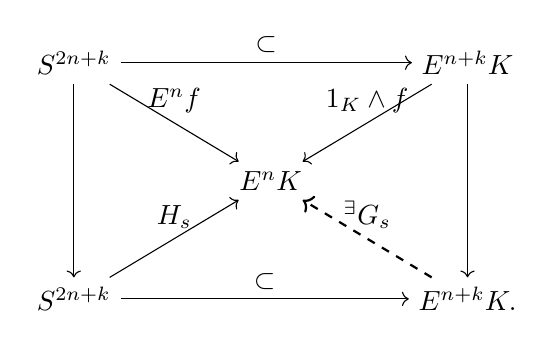
\begin{tikzpicture}[]
  \node (A) at (0,3) {$S^{2n+k}$};
  \node (B) at (5,3) {$E^{n+k}K$};
  \node (C) at (2.5,1.5) {$E^n K$};
  \node (D) at (0,0) {$S^{2n+k}$};
  \node (E) at (5,0) {$E^{n+k}K.$};
  \draw[->] (A) -- node[above] {$\subset$} (B);
  \draw[->] (A) -- node[above] {$E^n f$} (C);
  \draw[->] (A) -- node[left] {} (D);
  \draw[->] (B) -- node[above] {$1_K\wedge f$} (C);
  \draw[->] (B) -- node[right] {} (E);
  \draw[->] (D) -- node[above] {$H_s$} (C);
  \draw[->] (D) -- node[above] {$\subset$} (E);
  \draw[->, dashed, thick] (E) -- node[above] {${}^\exists G_s$} (C);
\end{tikzpicture}\\
\(H_0 = E^n f,\ H_1(S^{2n+k}) = e_0.\)

\noindent
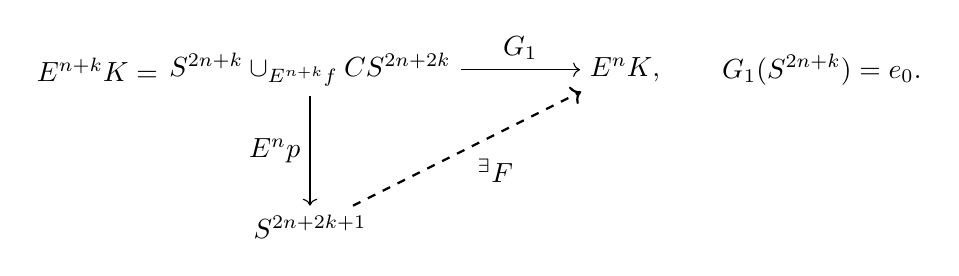
\begin{tikzpicture}[]
  \node (A) at (0,2) {$S^{2n+k}\cup_{E^{n+k}f}CS^{2n+2k}$};
  \node (B) at (4,2) {$E^{n}K$,};
  \node (C) at (0,0) {$S^{2n+2k+1}$};
  \node (D) at (-2.7,2) {$E^{n+k}K=$};
  \node (E) at (6.5,2) {$G_1(S^{2n+k}) = e_0.$};
  \draw[->] (A) -- node[above] {$G_1$} (B);
  \draw[->] (A) -- node[left] {$E^n p$} (C);
  \draw[->, dashed, thick] (C) -- node[below right] {${}^\exists F$} (B);
\end{tikzpicture}\\




\end{paracol}

\begin{paracol}{2}

\begin{lemma}\label{lem:3.5}
% Lem3.5
$\alpha\in\pis{n+k}{S^n}$, 整数 $h\ge0$ が, 
条件 \eqref{3.1} を満たすとする. \\
$\iota_K$ を $K$ の恒等写像のホモトピー類とし, 
さらに, $k\le 2n-2$ と仮定する. \\
\((1-(-1)^k)\,\Ex^{\,n+k-h}\alpha\) の任意の coextension
\(\gamma\ \in\ \pis{2n+2k-h+1}{\Ex^{n}K}\)
に対し, \\
ある元 $\alpha^{*}\in\pis{2n+2k+1}{S^{2n}}$ が存在して,
次が成り立つ.
\[
\iota_K \wedge \alpha
\;=\; (\Ex^{n+k}p)^{*}\!\Bigl(\, i_*\alpha^{*}\ +\ (-1)^{nk}\,\Ex^{h}\gamma \Bigr)
\in\ [\Ex^{n+k}K, Ex^{n}K]
\]
ここで, $i:S^{2n}\into\Ex^{n}K$ は 包含写像である. 
\end{lemma}

\textbf{Proof.}\ 
$1_K \wedge f$ と $F\circ \Ex^{n}p$ の間のホモトピーを $G_s$ とする. \\
$\phi_m:K\times S^m\to \Ex^{m}K$ ($m=n$ または $n+k$) を,
$\Ex^{m}K=K \wedge S^{m}$ の等化写像とする. \\
Prop3.1 により,
\[
\iota_n \wedge \alpha \;=\;(-1)^{nk}\,\Ex^n\alpha
= \alpha \wedge\ (-1)^{kn} \iota_n .
\]
このとき, ホモトピー
$A_s:(S^{2n+k},e_0)\to (S^{2n+k},e_0)$ で, 
次を満たすものが存在する.
\[
A_0=1_n \wedge f,\qquad A_1=f \wedge \tau.
\]
ここで,  $1_n$ は $S^n$ の恒等写像, $\tau:S^n\to S^n$ は
degree が $(-1)^{kn}$ の写像である. \\
次に, ホモトピー
\(G_s:\ \Ex^{n+k}K\ \longrightarrow\ \Ex^{n}K\)
を, 次の式で定める. \\
$S^{2n+k}$ の点 $\phi_{n+k,n}(x,y)$ に対して,
\[
G_s\bigl(\theta_{n+k,n}(x,y)\bigr)=
\begin{cases}
A_{2s}\!\bigl(\phi_{n+k,n}(x,y)\bigr), & 0\le s\le \tfrac12,\\[2pt]
\phi_{n}\!\bigl(d'(x,2s-1),\,\tau(y)\bigr), & \tfrac12\le s\le1.
\end{cases}
\]
また, $\Ex^{n+k}K$ の点 $\phi_{n+k}\!\bigl(d'(u,t),v\bigr)$ に対して,
\[
G_s\bigl(\phi_{n+k}(d'(u,t),v)\bigr)=
\begin{cases}
\phi_{n}\!\Bigl(d'\!\bigl(u,\,(2t-s)/(2-s)\bigr),\ f(v)\Bigr), & \tfrac{s}{2}\le t\le1,\\[3pt]
G_{s-2t}\!\bigl(\phi_{n,n+k}(f(u),v)\bigr), & 0\le t\le \tfrac{s}{2}.
\end{cases}
\]
\(G_s\) は well defined で, \\
$G_0=1_K \wedge f$ から,
$S^{2n+k}$ を一点につぶす写像 $G_1$ へのホモトピーになっている. \\
また, $\Ex^{n+k}p$ は $S^{2n+k}$ をつぶす写像なので, 
% --- CHAPTER III p.29 続き ---
$G_1=F\circ \Ex^{n+k}p$ を満たす写像
\[
F:\ S^{2n+2k+1}\longrightarrow \Ex^{n}K
\]
が一意に存在する. 
次の合成を考える. 
\[
\Ex^{n}p \circ F:\ S^{2n+2k+1}\longrightarrow S^{2n+k+1}
\]

\switchcolumn

\noindent
\textbf{(3.1).}\
\(\bigl(1-(-1)^k\bigr)\, \Ex^{\,n-h}\alpha \circ \Ex^{\,n+k-h}\alpha = 0.\)

\noindent
\textbf{Prop3.1.}\
\(
\alpha \wedge \beta
= (-1)^{(p+k)h} E^{q}\alpha \circ E^{p+k}\beta
= (-1)^{ph} E^{p}\beta \circ E^{q+h}\alpha .
\)


\end{paracol}

\begin{paracol}{2}

\noindent
上記の定義式を用いた直接計算から, 
\(E^n p\circ F\) は, 次の式で与えられる. 
\[
(E^n p\circ F)(\phi_{n+k+1, n+k}(d_{n+k}(u, t), v))=
\begin{cases}
\phi_{n+k+1, n}(d_{n+k}(u, 2t-1), f(v)), & \frac{1}{2}\le t\le1,\\[3pt]
e_0, & \frac{1}{4}\le t\le \frac{1}{2},\\[3pt]
\phi_{n+k+1, n+k}(d_{n+k}(x, 1-4t), \tau(y)), & 0\le t\le \frac{1}{4}.
\end{cases}
\]
ここで, 
\(\phi_{n+k, n}(x, y) = \phi_{n, n+k}(f(u), v)\) である. \\
この写像は, \((n+k+1)\) 番目の座標 $t$ に関する 3 つの写像の和
\(H_1 + (H_0 - H_2)\) で, \\
ホモトピー類が,
\([E^n p\circ F] = [H_1] + [H_0] - [H_2]\) 
となるものと考えることができる. \\
ここで, \(H_0\) は自明な写像で, $H_1,H_2$ は次で与えられる. 
\[
\begin{aligned}
H_1\bigl(\phi_{n+k+1,n+k}(d_{n+k}(u,t),v)\bigr)
&=\phi_{n+k+1,n}\bigl(d_{n+k}(u,t),\,f(v)\bigr),\\
H_2\bigl(\phi_{n+k+1,n+k}(d_{n+k}(u,t),v)\bigr)
&=\phi_{n+k+1,n}\bigl(d_{n+k}(u,t),\,\tau(y)\bigr).
\end{aligned}
\]
明らかに, $[H_0]=0$ であり, 
\[
[H_1] = [\,1_{n+k+1} \wedge f\,]\ 
=\ \iota_{n+k+1} \wedge \alpha
 = (-1)^{(n+k+1)k}\Ex^{n+k+1}\alpha\
=\ (-1)^{kn}E^{n+k+1}\alpha .
\]
また, degree \((-1)^k\) の自己同相写像 
\(\sigma:S^{2n+k+1}\to S^{2n+k+1}\) を, \\
\[
\sigma(\psi(x_1,\ldots,x_{n+k}, t, y_1,\ldots,y_n))
= \psi(x_1,\ldots, x_n, t, x_{n+1},\ldots,x_{n+k} y_1,\ldots,y_n)
\]
で与えるとき, $H_2$ に対して次が成り立つことが, 直接的に確かめられる.
\[
[H_2] = (\iota_{n+k+1} \wedge (-1)^{kn} \iota_n) \circ (-1)^{k}\iota_{2n+k+1}
\circ (E\alpha \wedge \iota_{n+k})
 = (-1)^{kn+k}E^{n+k+1}\alpha .
\]
よって, 
\[
(\Ex^{n}p)_*\,[F] = (-1)^{kn}\bigl(1-(-1)^k\bigr)\,\Ex^{n+k+1}\alpha .
\]
一方, coextension の定義から,
\[
(\Ex^{n-h}p)_*(\gamma) = \bigl(1-(-1)^k\bigr)\,\Ex^{n+k-h+1}\alpha .
\]
(1.6) を用いれば,
\[
(\Ex^{n}p)_*\,\Ex^{h}\gamma
=\Ex^{h}\!\bigl((\Ex^{n-h}p)_*\gamma\bigr)
=\bigl(1-(-1)^k\bigr)\,\Ex^{n+k+1}\alpha,
\]
\[
(\Ex^{n}p)_*\bigl(\,[F]\ -\ (-1)^{kn}\Ex^{h}\gamma\,\bigr) = 0 .
\]
仮定 $k\le 2n-2$ から, 
$2n+2k+1\le (2n+k)+(2n-1)$ が成り立つ. \\
対 $(\Ex^{n}K, S^{2n})$ は, $(2n+k)$-connected であり, 
$S^{2n}$ は $(2n-1)$-connected である. \\
したがって, \cite{BlakersMassey1952} Theorem2 より, 次の誘導準同型は同型である.
\[
(\Ex^{n}p)_*\ :\ 
\pi_{2n+2k+1}\bigl(\Ex^{n}K,S^{2n}\bigr)\
\longrightarrow\
\pi_{2n+k+1}\bigl(S^{2n+k+1}\bigr).
\]

\switchcolumn

\noindent
\textbf{(1.6).}\
\(\text{0).}\ 
f\simeq g:X\to Y \text{ は, }
E^n f\simeq E^n g \text{ を導く.}\)\\
\([f]\mapsto [E^n f] \text{ は, } 
E^n : [X,Y] \to [E^n X, E^n Y] \text{ を定める.}\)\\
\(\text{i).}\ 
E^n(E^m\alpha) = E^{n+m}\alpha,
\text{ for } \alpha\in [X,Y].\)\\
\(\text{ii).}\
E^n(g\circ f) = E^n g\circ E^n f,\quad
E^n(\beta\circ\alpha) = E^n\beta\circ E^n\alpha.\)

\noindent
\textbf{
\cite{BlakersMassey1952}
A.~L.~Blakers and W.~S.~Massey,}
\newblock The homotopy groups of a triad II,
\newblock Ann. of Math., {\bf 55} (1952), 192--201.

\noindent
\textbf{Th2.}\ \(\pi_i(X,A)=0\ (i<n),\ \pi_i(A)=0\ (i<m),\ 
p:(X,A)\to(X/A,*),\)\\
\(\Longrightarrow p_*:\pis{i}{X,A}\to\pis{i}{X/A}\)
は, \(i<n+m-1\) で同型, \\
% \(\pis{i}{S^m_\infty, S^m_{p-1}}=0\ (i<pm),\ 
% \pis{i}{S^m_{p-1}} = 0\ (i<m).\)


\end{paracol}

\begin{paracol}{2}

次の図式において, 横の列は完全列である. 
% --- CHAPTER III p.30 ---
\[
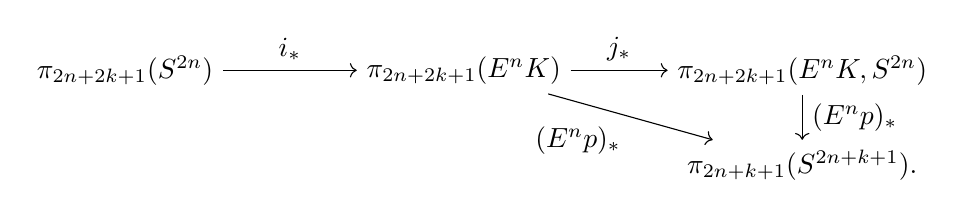
\begin{tikzpicture}[baseline=(current bounding box.center)]
  \node (A) at (0,1.2) {$\pis{2n+2k+1}{S^{2n}}$};
  \node (B) at (4.3,1.2) {$\pis{2n+2k+1}{\Ex^{n}K}$};
  \node (C) at (8.6,1.2) {$\pis{2n+2k+1}{\Ex^{n}K,S^{2n}}$};
  \node (D) at (8.6,0)   {$\pis{2n+k+1}{S^{2n+k+1}} .$};
  \draw[->] (A)--node[above] {$\ i_*\ $}(B);
  \draw[->] (B)--node[above] {$\ j_*\ $}(C);
  \draw[->] (C)--node[right] {$(\Ex^{n}p)_*\ $}(D);
  \draw[->] (B) to[right=18] node[below left] {$(E^n p)_{*}$} (D);
\end{tikzpicture}
\]
\((\Ex^{n}p)_*\bigl([F]-(-1)^{kn}\Ex^{h}\gamma\bigr)=0\) 
であることから, \\
\([F]-(-1)^{kn}\Ex^{h}\gamma=\iota_*\,\alpha^{*}\)
となる $\alpha^{*}\in\pis{2n+2k+1}{S^{2n}}$ が存在する. ゆえに,
\[
\iota_K \wedge \alpha \;=\; [G_0]
 = [G_1]\;=\; (\Ex^{n+k}p)^* [F]
\;=\;(\Ex^{n+k}p)^{*}\!\Bigl(\iota_*\alpha^{*}+(-1)^{kn}\Ex^{h}\gamma\Bigr) .
\]
以上で, Lemma が示された. 
\qed

\switchcolumn

\end{paracol}

\begin{paracol}{2}

\begin{theorem}\label{thm:3.6}
% Th3.6
$\alpha\in\pis{n+k}{S^{n}}$, $h\ge0$ が \eqref{3.1} を満たすとする.\\ 
さらに, $k\le 2n-2$ と仮定する.
このとき,
\(\alpha^{*}\in\pis{2n+2k+1}{S^{2n}}\)
が存在して, \\
\(\beta\circ \Ex^{\ell}\alpha=0\)
を満たす任意の $\beta\in\pis{n+\ell}{S^{n}}$ に対して, 
\[
\begin{align*}
  \Ex^{n}\beta \circ \Ex^{t}\alpha^{*} 
  & \in (-1)^{km+kt+t}\,\todai[n+k]{\Ex^{m}\alpha,\ 
  \Ex^{n+k}\beta,\ \Ex^{n+k+t}\alpha}\\
  & + (-1)^{kn+h+t+1}\,\todai[h+t]{\Ex^{n}\beta,\ 
  \Ex^{n+t}\alpha,\ (1-(-1)^k)\Ex^{n+k+t}\alpha}\ .
\end{align*}
\]
さらに,
\((1-(-1)^k)\Ex^{n+h+1}\alpha=0\), 特に \(k\) が偶数のとき, 
\[
\Ex^{n}\beta\circ \Ex^{t}\alpha^{*}\ \in\
(-1)^{km+kt+t}\,\todai[n+k]{\Ex^{m}\alpha,\ \Ex^{n+k}\beta,\ \Ex^{n+k+t}\alpha}\ .
\]
\end{theorem}

\textbf{Proof.}\ 
$\beta\circ \Ex^{t}\alpha=0$ なので, $\beta$ の $\Ex^{n}K$ への extension
\(\ext{\beta}\in \hs{E^t K}{S^{m}}\)
が存在する. \\
\(\alpha'=\Ex^{t}\alpha\) とし, 
(1.16) により, \(\Ex^{n}K\) と \(S^{n+t}\cup_{\alpha'}CS^{n+k+t}\)
を同一視する. \\
\(p':\Ex^{n}K = S^{n+t}\cup_{\alpha'}CS^{n+k+t} \to S^{n+k+t+1}\)
を (1.17) の中で定義された写像とすると, 
\[
\sigma(\psi_{n+k+t+1}(t_1,\cdots,t_{n+k+t},t))
=\psi_{n+k+t+1}(t_1,\cdots,t_{n+k},t,t_{n+k+1},\cdots,t_{n+k+t})
\]
により与えられる, 次数 \((-1)^{t}\) の自己同相写像
$\sigma:S^{n+k+t+1}\to S^{n+k+t+1}$
に対して, 
\[
p'=\sigma\circ \Ex^{t}p
\]
が成り立つ. 
次に, reduced join 
\[
\ext{\beta} \wedge \alpha\ \in\ [\Ex^{n+k+t}K, S^{m+n}]
\]
について考える. \\

\switchcolumn

\noindent
\textbf{(3.1).}\
\(\bigl(1-(-1)^k\bigr)\, \Ex^{\,n-h}\alpha \circ \Ex^{\,n+k-h}\alpha = 0.\)

\noindent
\textbf{(1.17).}\
\(p:X\cup_\gamma CW\to EW,\qquad
p(d'_W(w, t)) := d_W(w, t),\quad
p(X) := x_0.\)

\end{paracol}

\begin{paracol}{2}

\noindent
まず, 次を得る. 
\[
\begin{align*}
\ext{\beta} \wedge \alpha
&= (\ext{\beta} \circ E^t \iota_K)\ \wedge (\iota_n \circ \alpha) \\
&= (\ext{\beta} \wedge \iota_n) \circ ((\iota_K \wedge \iota_t) \wedge \alpha)
&&\text{by (1.5)}\\
&= \Ex^{n}\ext{\beta}\ \circ\
(\ \iota_K \wedge \alpha \wedge (-1)^{kt}\,\iota_t\ )
&&\text{by Prop \ref{prop:3.1}}\\
&= E^n\ext{\beta} \circ (-1)^{kt} E^t ((E^{n+k}p)^{*}(i_*\alpha^* + (-1)^{kn}E^h \gamma))
&&\text{by Lem \ref{lem:3.5}}\\
&= (-1)^{kt}\Ex^{n}\ext{\beta}\circ(\Ex^{n+k+t}p)^{*}(\Ex^{t}i_*\alpha^* + (-1)^{kn}E^{h+t}\gamma)
&&\text{by (1.6)} \\
&= (-1)^{kt}(\Ex^{n+k}p')^{*}(E^{n+k}\sigma)^{*}
( \Ex^{n}\beta\circ\Ex^{t}\alpha^{*}
\ +\ (-1)^{kn}\Ex^{n}\ext{\beta}\circ\Ex^{h+t}\gamma )\\
&= (-1)^{(k+1)t}(E^{n+k}p')^{*}
(E^n\beta\circ E^t\alpha^* + (-1)^{kn}E^n\ext{\beta}\circ E^{h+t}\gamma) .
\end{align*}
\]
Prop1.7 により, 
\[
E^n\ext{\beta}\circ E^{t+h}\gamma
\in (-1)^{h+t}\todai[h+t]{E^n\beta, E^{n+t}\alpha, (1-(-1)^k)E^{n+t+k}\alpha} .
\]
% --- CHAPTER III p.31 ---
また, 
\[
\begin{align*}
\ext{\beta} \wedge \alpha
&= (\iota_m \circ \ext{\beta}) \wedge (\alpha \circ \iota_{n+k})\\
&= (\iota_m \wedge \alpha) \circ (\ext{\beta} \wedge \iota_{n+k}) && \text{by (1.5)}\\
&= (-1)^{km}\Ex^{m}\alpha \circ \Ex^{n+k}\ext{\beta} && \text{by Prop3.1}\\
&= (-1)^{km}(\Ex^{m}\alpha \circ\ \Ex^{n+k}\ext{\beta}) .
\end{align*}
\]
Prop1.9 より, 
\[
(E^{n+k}p')^{*}\lambda = E^m\alpha\circ E^{n+k}\ext{\beta}
\]
を満たす任意の元 \(\lambda\) は, 
\(\todai[n+k]{E^m\alpha, E^{n+k}\beta, E^{n+k+t}\alpha}\)
に属する. 
特に, 最初の計算により,
\[
\lambda = (-1)^{km+(k+1)t} (\Ex^{n}\beta\circ \Ex^{t}\alpha^* 
+ (-1)^{kn}\Ex^{n}\ext{\beta}\circ \Ex^{h+t}\gamma)
\]
は, この条件を満たしている. 
したがって, 
\[
(-1)^{km+(k+1)t}\Ex^{n}\beta\circ \Ex^{t}\alpha^{*}
+(-1)^{kn}\Ex^{n}\ext{\beta}\circ \Ex^{h+t}\gamma
\ \in\
\todai[n+k]{\Ex^{m}\alpha,\ \Ex^{n+k}\beta,\ \Ex^{n+k+t}\alpha}.
\]
\(\Ex^{n}\ext{\beta}\circ \Ex^{h+t}\gamma\)
に関する上の結果と合わせると, 
\[
\begin{align*}
\Ex^{n}\ext{\beta}\circ \Ex^{t}\alpha^{*}
&\in (-1)^{km+(k+1)t}\todai[n+k]{\Ex^{m}\alpha, \Ex^{n+k}\beta, E^{n+k+t}\alpha}\\
&+ (-1)^{kn+h+t+1}\todai[h+t]{E^n\beta, E^{n+t}\alpha, (1-(-1)^k)E^{n+k+t}\alpha} .
\end{align*}
\]
$(1-(-1)^k)\Ex^{n+h+1}\alpha=0$ の場合を考える. \\
Lem3.5 の中で, 
\((1-(-1)^k)E^{n+k+1}\alpha\) の coextension \(\gamma\) 
として, \(0\) を選ぶことができる. \\ 
このとき, 上の議論の中で, \(E^n\ext{\beta}\circ E^{h+t}\gamma\) の項は消える. 
よって, 
\[
E^n\beta\circ E^t\alpha^{*}
\in (-1)^{km+(k+1)t}\todai[n+k]{E^m\alpha, E^{n+k}\beta, E^{n+k+t}\alpha}
\]
であり, Th3.6 が証明された. 
\qed

\switchcolumn

\noindent
\textbf{(1.5).}\
\textbf{i).}\ \((\alpha\wedge\beta)\wedge\gamma 
  = \alpha\wedge(\beta\wedge\gamma).\)\\
\textbf{ii).}\ \((\alpha'\circ\alpha)\wedge(\beta'\circ\beta)
  = (\alpha'\wedge\beta')\circ(\alpha\wedge\beta).\)

\noindent
\textbf{Prop3.1.}\
\(
\alpha \wedge \beta
= (-1)^{(p+k)h} E^{q}\alpha \circ E^{p+k}\beta
= (-1)^{ph} E^{p}\beta \circ E^{q+h}\alpha .
\)

\noindent
\textbf{Lem3.5.}\
$\alpha\in\pis{n+k}{S^n}$, 整数 $h\ge0$ が, 
条件 \eqref{3.1} を満たすとする. \\
$\iota_K$ を $K$ の恒等写像のホモトピー類とし, 
さらに, $k\le 2n-2$ と仮定する. \\
\((1-(-1)^k)\,\Ex^{\,n+k-h}\alpha\) の任意の coextension
\(\gamma\ \in\ \pis{2n+2k-h+1}{\Ex^{n}K}\)
に対し, \\
ある元 $\alpha^{*}\in\pis{2n+2k+1}{S^{2n}}$ が存在して,
次が成り立つ.\\
\(
\iota_K \wedge \alpha
\;=\; (\Ex^{n+k}p)^{*}\!\Bigl(\, i_*\alpha^{*}\ +\ (-1)^{nk}\,\Ex^{h}\gamma \Bigr)
\in\ [\Ex^{n+k}K, Ex^{n}K]
\)\\
ここで, $i:S^{2n}\into\Ex^{n}K$ は 包含写像である. 

\noindent
\textbf{(1.6).}\
\(\textbf{0).}\ 
f\simeq g:X\to Y \text{ は, }
E^n f\simeq E^n g \text{ を導く.}\)\\
\([f]\mapsto [E^n f] \text{ は, } 
E^n : [X,Y] \to [E^n X, E^n Y] \text{ を定める.}\)\\
\(\textbf{i).}\ 
E^n(E^m\alpha) = E^{n+m}\alpha,
\text{ for } \alpha\in [X,Y].\)\\
\(\textbf{ii).}\
E^n(g\circ f) = E^n g\circ E^n f,\quad
E^n(\beta\circ\alpha) = E^n\beta\circ E^n\alpha.\)

\noindent
\textbf{Prop1.9.}\
$\alpha,\beta,\gamma$ は, \textnormal{Prop1.7} と同様とする. 
$\overline\beta\in[X\cup_f CW, Y]$ を,\\
$\beta$ の \emph{extension} とするとき,
ある $\lambda\in[\Ex^{n+1}W, Z]$ が存在して, 次を満たす.\\
\(
(\Ex^n p)^*\lambda=\alpha\circ \Ex^n\overline\beta.
\)\\
このような $\lambda$ 全体の集合は,
\(
[\Ex^{n+1}X, Z]\circ \Ex^{n+1}\gamma
\)
の coset であり, 特に, 次が成り立つ.\\
\(
\{\lambda\}\ \subset\ \{\alpha,\ \Ex^n\beta,\ \Ex^n\gamma\}_n .
\)\\
逆に, $\{\alpha,\Ex^n\beta,\Ex^n\gamma\}_n$ の任意の元 $\lambda$ に対し, 
適当な extension $\overline\beta$ が存在して,
次が成り立つ.\\
\(
(\Ex^n p)^*\lambda=\alpha\circ \Ex^n\overline\beta.
\)

\noindent
\textbf{Th3.6.}\
$\alpha\in\pis{n+k}{S^{n}}$, $h\ge0$ が \eqref{3.1} を満たすとする.\\ 
さらに, $k\le 2n-2$ と仮定する.
このとき,
\(\alpha^{*}\in\pis{2n+2k+1}{S^{2n}}\)
が存在して, \\
\(\beta\circ \Ex^{\ell}\alpha=0\)
を満たす任意の $\beta\in\pis{n+\ell}{S^{n}}$ に対して, \\
\(\Ex^{n}\beta \circ \Ex^{t}\alpha^{*}
\in (-1)^{km+kt+t}\,\todai[n+k]{\Ex^{m}\alpha,\ 
  \Ex^{n+k}\beta,\ \Ex^{n+k+t}\alpha}\)\\
\(+ (-1)^{kn+h+t+1}\,\todai[h+t]{\Ex^{n}\beta,\ 
  \Ex^{n+t}\alpha,\ (1-(-1)^k)\Ex^{n+k+t}\alpha}\ .\)\\
さらに,
\((1-(-1)^k)\Ex^{n+h+1}\alpha=0\), 特に \(k\) が偶数のとき, \\
\(
\Ex^{n}\beta\circ \Ex^{t}\alpha^{*}\ \in\
(-1)^{km+kt+t}\,\todai[n+k]{\Ex^{m}\alpha,\ \Ex^{n+k}\beta,\ \Ex^{n+k+t}\alpha}\ .
\)



\end{paracol}

\begin{paracol}{2}

\begin{corollary}\label{cor:3.7}
% Cor3.7
整数 $r$ をとる. $\beta\in\pis{m+k}{S^m}$, $(k>0)$ が $r\beta=0$ を満たすとき,
\[
\todai[1]{\,r\,\iota_{m+1},\ \Ex\beta,\ r\,\iota_{m+k+1}\,}
\begin{cases}
\equiv 0, & r\not\equiv 2 \pmod 4,\\[4pt]
\ni\Ex\beta\circ \eta_{m+k+1}, & r\equiv 2 \pmod 4 .
\end{cases}
\]
ここで, $\eta_{m+k+1}$ は $\pis{m+k+2}{S^{m+k+1}}\cong\mathbb{Z}_2$ の生成元とする. 
\end{corollary}

\textbf{Proof.}\ 
これを証明するために, 次の事実を用いる (Chapter V 参照) :
\[
\pis{n+1}{S^n}\cong\mathbb{Z}_2,\ (n\ge3) .
\]
この生成元を $\eta_n$ とし, $\eta_{n+1}=E \eta_{n}$とすると, 
\(\eta_n\circ\eta_{n+1}\) は \(\pis{n+2}{S^n}\) の生成元である. \\
さらに, Toda bracket について, 次が成り立つ. 
\[
\toda{\,2\iota_n,\ \eta_n,\ 2\iota_{n+1}\,}
=\{\eta_n\circ\eta_{n+1}\}.
\]
(\cite{Toda1952}, Chapter VIII 例2 を見よ. )\\
Th3.6 において, $\alpha=r\,\iota_{m+1}$ と置くと, 
ある \(r\) のみによって決まる整数 $t=t(r)$ が存在し, 
\[
\Ex\beta\circ t\eta_{m+k+1}
\ \in\ \todai[1]{\,r\iota_{m+1},\ \Ex\beta,\ r\iota_{m+k+1}\,}.
\]
$r$ が奇数のとき, 
\[
E\beta\circ\eta_{m+k+1}
= r(E\beta\circ\eta_{m+k+1})
\in r (\pis{m+k+2}{S^{m+1}}) .
\]
よって, \(E\beta\circ\eta_{m+k+1}\) は, 
\(\todai[1]{r\iota_{m+1}, E\beta, r\iota_{m+k}}\) 
の coset に含まれるので, 
\[
\todai[1]{r\iota_{m+1}, E\beta, r\iota_{m+k}} \equiv 0.
\]

% --- CHAPTER III p.32 ---
%  (前段の系 \ref{cor:3.7} の偶奇場合わけのまとめ) 
次に, $r$ を偶数とし, $r=2s$ と置く. 
Prop1.2 により, 
\[
s^2(\eta_n\circ\eta_{n+1})
\in s\iota_n\circ\toda{2\iota_n, \eta_n, 2\iota_{n+1}}\circ s\iota_{n+2}
\subset \toda{r\iota_n, \eta_n, r\iota_{n+1}} .
\]
また, 
\(t(\eta_n\circ\eta_{n+1}) \in \toda{r\iota_n, \eta_n, r\iota_{n+1}}\)
であり, これはただ1つの元だけから成る. \\
よって, 
\(
s^2(\eta_n\circ\eta_{n+1}) = t(\eta_n\circ_{n+1})
\)
なので, \(s^2\equiv t\mod 2\) である. \\
$s$ が偶数 (すなわち $r\equiv0\pmod4$) のとき, 
\[
\Ex\beta\circ t\,\eta_{m+k+1}=0 .
\]
$s$ が奇数 ($r\equiv2\pmod4$) のとき, 
\[
\Ex\beta\circ t\,\eta_{m+k+1}=\Ex\beta\circ \eta_{m+k+1} .
\]
以上より, Cor3.7 が示された. 
\qed

\switchcolumn

\noindent
\textbf{
\cite{Toda1952}
H.~Toda,}
\newblock Generalized Whitehead products and homotopy groups of spheres,
\newblock Jour. of Inst. Poly. Osaka City Univ., {\bf 3} (1952), 43--82.

\noindent
\textbf{Th3.6.}\
$\alpha\in\pis{n+k}{S^{n}}$, $h\ge0$ が \eqref{3.1} を満たすとする.\\ 
さらに, $k\le 2n-2$ と仮定する.
このとき,
\(\alpha^{*}\in\pis{2n+2k+1}{S^{2n}}\)
が存在して, \\
\(\beta\circ \Ex^{\ell}\alpha=0\)
を満たす任意の $\beta\in\pis{n+\ell}{S^{n}}$ に対して, \\
\(\Ex^{n}\beta \circ \Ex^{t}\alpha^{*}
\in (-1)^{km+kt+t}\,\todai[n+k]{\Ex^{m}\alpha,\ 
  \Ex^{n+k}\beta,\ \Ex^{n+k+t}\alpha}\)\\
\(+ (-1)^{kn+h+t+1}\,\todai[h+t]{\Ex^{n}\beta,\ 
  \Ex^{n+t}\alpha,\ (1-(-1)^k)\Ex^{n+k+t}\alpha}\ .\)\\
さらに,
\((1-(-1)^k)\Ex^{n+h+1}\alpha=0\), 特に \(k\) が偶数のとき, \\
\(
\Ex^{n}\beta\circ \Ex^{t}\alpha^{*}\ \in\
(-1)^{km+kt+t}\,\todai[n+k]{\Ex^{m}\alpha,\ \Ex^{n+k}\beta,\ \Ex^{n+k+t}\alpha}\ .
\)

\noindent
\textbf{Prop1.2.}\
\textbf{0).}\ $\alpha$, $\beta$, $\gamma$ のうち, いずれかが $0$ なら,\\
\(
\{\alpha,\ \Ex^n\beta,\ \Ex^n\gamma\}_n\equiv0.
\)\\
\textbf{i).}\ $\alpha\circ \Ex^n\beta=\beta\circ\gamma=0$ のとき,\\
\(
\{\alpha,\ \Ex^n\beta,\ \Ex^n\gamma\}_n\circ\Ex^{n+1}\delta\ \subset\ \{\alpha,\Ex^n \beta, \Ex^n(\gamma\circ\delta)\}_n.
\)\\
\textbf{ii).}\ $\alpha\circ \Ex^n\beta=\beta\circ\gamma\circ\delta=0$ のとき,\\
\(
\{\alpha,\ \Ex^n\beta,\ \Ex^n(\gamma\circ\delta)\}_n\ \subset\ \{\alpha,\ \Ex^n(\beta\circ\gamma),\ \Ex^n\delta\}_n .
\)\\
\textbf{iii).}\ $\alpha\circ\Ex^n\beta\circ\Ex^n\gamma=\gamma\circ\delta=0$ なら,\\
\(
\{\alpha\circ\Ex^n\beta,\ \Ex^n\gamma,\ \Ex^n\delta)\}_n\ \subset\ \{\alpha,\ \Ex^n(\beta\circ\gamma),\ \Ex^n\delta\}_n .
\)\\
\textbf{iv).}\ $\beta\circ\Ex^n\gamma=\gamma\circ\delta=0$ のとき,\\
\(
\alpha\circ\{\beta,\ \Ex^n\gamma,\ \Ex^n\delta\}_n\ \subset\ \{\alpha\circ\beta,\ \Ex^n\gamma,\ \Ex^n\delta\}_n .
\)



\end{paracol}

\begin{paracol}{2}

\medskip
\noindent
(2.11) の完全列の結果として Freudenthal の懸垂定理を得る：
\begin{equation}\label{3.2}
% (3.2)
\Ex: \pis{i}{S^m} \longrightarrow \pis{i+1}{S^{m+1}}
\quad\text{は, } i<2m-1 \text{で同型, } i=2m-1 \text{で全射である. }
\end{equation}

球面の $k$ 次安定ホモトピー群を
\[
G_k\ :=\ \lim_{n\to\infty}\ \pis{n+k}{S^n}
\]
と書き, 射影を
\[
\Ex^\infty:\ \pis{n+k}{S^n}\ \longrightarrow\ G_k
\]
で表す. (3.2) から,
\begin{equation}\label{3.3}
% (3.3)
\Ex^\infty:\ \pis{n+k}{S^n}\ \xrightarrow{\;\;}\ G_k
\quad\text{は, } n>k+1 \text{で同型, } n=k+1 \text{で全射である. }
\end{equation}

(1.6) より,
\(\Ex^{m}(\alpha\circ\beta)=\Ex^{m}\alpha\circ\Ex^{m}\beta\)
なので, 合成
\[
\circ:G_k\times G_h \rightarrow G_{k+h}
\]
が, \(E^\infty(\alpha\circ\beta)=E^\infty\alpha\circ E^\infty\beta\) 
により定義される. \\
(1.7) または (2.1) は, 合成が stable の範囲では bilinear であることを示している. 
\[
\alpha\circ(\beta_1\pm\beta_2)=\alpha\circ\beta_1\pm\alpha\circ\beta_2,\qquad
(\alpha_1\pm\alpha_2)\circ\beta=\alpha_1\circ\beta\pm\alpha_2\circ\beta .
\]
Prop3.1 は, anti-commutativity を示している. 
\begin{equation}\label{3.4}
% (3.4)
\alpha\circ\beta=(-1)^{kh}\,\beta\circ\alpha,
\qquad(\alpha\in G_k,\ \beta\in G_h) .
\end{equation}

\medskip
\noindent
\[
\alpha\in G_k,\quad \beta\in G_h,\quad \gamma\in G_\ell,\qquad
\alpha\circ\beta=\beta\circ\gamma=0
\]
に対する, stable Toda bracket 
\[
\langle \alpha,\beta,\gamma\rangle 
\in G_{k+h+\ell+1}(\alpha\circ G_{h+\ell+1} + \gamma\circ G_{k+h+1}) .
\]
を以下の様に定義する. 
十分大きな $n$ をとれば, 
\[
\alpha'\in\pis{n+k}{S^n},\ 
\beta'\in\pis{n+k+h}{S^{n+k}},\
\gamma'\in\pis{n+k+h+\ell}{S^{n+k+h}}
\]
が存在して, 
\(
\alpha=\Ex^\infty\alpha',\
\beta=\Ex^\infty\beta',\
\gamma=\Ex^\infty\gamma'
\)
と書ける. \\
このとき, 
\(\langle \alpha,\beta,\gamma\rangle\)
を, 次で定義する.
\[
\langle \alpha,\beta,\gamma\rangle
\ :=\ \Ex^\infty (-1)^{\,n-1}\ \toda{\alpha',\beta',\gamma'}.
\]
Prop1.3 により, この定義は $n$ によらず well-defined である. 

\switchcolumn

\noindent
\textbf{(2.11).}\
\(\cdots\ \longrightarrow\ 
\pi_i(S^m)\xrightarrow{\,E\,}\pi_{i+1}(S^{m+1})\xrightarrow{\,H\,}
\pi_{i+1}(S^{2m+1})\xrightarrow{\,\Delta\,}\pi_{i-1}(S^m)\xrightarrow{\,E\,}\cdots.\)

\noindent
\textbf{(1.6).}\
\(\textbf{0).}\ 
f\simeq g:X\to Y \text{ は, }
E^n f\simeq E^n g \text{ を導く.}\)\\
\([f]\mapsto [E^n f] \text{ は, } 
E^n : [X,Y] \to [E^n X, E^n Y] \text{ を定める.}\)\\
\(\textbf{i).}\ 
E^n(E^m\alpha) = E^{n+m}\alpha,
\text{ for } \alpha\in [X,Y].\)\\
\(\textbf{ii).}\
E^n(g\circ f) = E^n g\circ E^n f,\quad
E^n(\beta\circ\alpha) = E^n\beta\circ E^n\alpha.\)

\noindent
\textbf{(1.7).}\
\(f:Y\to Z,\ g:W\to X \text{ に対して, 次は準同型である.}\)\\
\(
f_*:[EX, Y] \to [EX,Z],\quad Eg^*:[EX,Y]\to[EW,Y].
\)

\noindent
\textbf{(2.1).}\
\(\alpha\circ(\beta_1\pm\beta_2) =\alpha\circ\beta_1\ \pm\ \alpha\circ\beta_2,\)\\
\((\alpha_1\pm\alpha_2)\circ E\beta =\alpha_1\circ E\beta\ \pm\ \alpha_2\circ E\beta,\)\\
特に, 任意の整数 $k$ に対して,\\
\(
k(\alpha\circ\beta)=\alpha\circ(k\beta),\
k(\alpha\circ E\beta)=(k\alpha)\circ E\beta.
\)

\noindent
\textbf{Prop3.1.}\
\(
\alpha \wedge \beta
= (-1)^{(p+k)h} E^{q}\alpha \circ E^{p+k}\beta
= (-1)^{ph} E^{p}\beta \circ E^{q+h}\alpha .
\)

\noindent
\textbf{Prop1.3.}\
任意の $n\ge 0$ に対し,\\
\(
-\Omega_0\bigl\{\alpha,\ \Ex^{n+1}\beta,\ \Ex^{n+1}\gamma\bigr\}_{n+1}
=
\bigl\{\Omega_0\alpha,\ \Ex^{n}\beta,\ \Ex^{n}\gamma\bigr\}_n \ ,
\)\\
\(
-\Ex\{\alpha,\ \Ex^n\beta,\ \Ex^n\gamma\}_n
\subset
\bigl\{E\alpha,\ \Ex^{n+1}\beta,\ \Ex^{n+1}\gamma\bigr\}_{n+1}.
\)





\end{paracol}

\begin{paracol}{2}


\noindent
通常の Toda bracket のいくつかの性質が, stable の場合に翻訳される. 

Prop1.2 から, 次が成り立つ. 
% 0) zero law
\begin{equation}\label{3.prop-zero}
% (3.5)
\raisetag{3ex}
  \begin{aligned}[t]
    \text{0).}\ & \todas{\alpha, \beta, \gamma}\equiv 0,
    \qquad\text{ ($\alpha,\beta,\gamma$ のいずれかが $0$ のとき) }.
    \qquad\qquad\qquad\qquad\qquad\\
    \text{i).}\ & \todas{\alpha, \beta, \gamma}\circ\delta
    \subset \todas{\alpha, \beta, \gamma\circ\delta}\\
    \text{ii).}\ & \todas{\alpha, \beta, \gamma\circ\delta}
    \subset \todas{\alpha, \beta\circ\gamma, \delta}\\
    \text{iii).}\ & \todas{\alpha\circ\beta, \gamma, \delta}
    \subset \todas{\alpha, \beta\circ\gamma, \delta}\\
    \text{iv).}\ & \alpha\circ\todas{\beta, \gamma, \delta}
    \subset (-1)^k\todas{\alpha\circ\beta, \gamma, \delta},\ \alpha\in G_k .
  \end{aligned}
\end{equation}

Prop1.4 から, 次が成り立つ. 
% 3.6) composition out the right (anti-derivation law)
\begin{equation}\label{3.6-stable}
\todas{\alpha,\beta,\gamma}\circ\delta
 = (-1)^{k+1}\,\alpha\circ\todas{\beta,\gamma,\delta},
\qquad \alpha\in G_k.
\end{equation}

% 3.7) Jacobi-type relation
Prop1.5 から, 次が成り立つ. 
\(\alpha\in G_k,\ \beta\in G_h\) のとき, 
\begin{equation}\label{3.7-stable}
% (3.8)
0\ \in\
\todas{\todas{\alpha,\beta,\gamma},\,\delta,\,\varepsilon}
\ +\ (-1)^{k}\,\todas{\alpha,\,\todas{\beta,\gamma,\delta},\,\varepsilon}
\ +\ (-1)^{k+h}\,\todas{\alpha,\,\beta,\,\todas{\gamma,\delta,\varepsilon}}.
\end{equation}

% 3.8) additivity / bilinearity
Prop1.6 から, 次が成り立つ. 
\begin{equation}\label{3.8-stable}
% (3.8)
\raisetag{3ex}
\begin{aligned}[t]
\todas{\alpha,\beta,\gamma}\ +\ \todas{\alpha,\beta,\gamma'}\ &\supset\
\todas{\alpha,\beta,\,\gamma+\gamma'},\\
\todas{\alpha,\beta,\gamma}\ +\ \todas{\alpha,\beta',\gamma}\ &=\
\todas{\alpha,\,\beta+\beta',\,\gamma},\\
\todas{\alpha,\beta,\gamma}\ +\ \todas{\alpha',\beta,\gamma}\ &\supset\
\todas{\,\alpha+\alpha',\,\beta,\,\gamma}.
\end{aligned}
\end{equation}

% 3.9) relations coming from reduced join symmetry (Proposition 3.4)
Prop3.4 から, 次が成り立つ. 
\(\alpha\in G_k,\ \beta\in G_h,\ \gamma\in G_\ell\) のとき, 
\begin{equation}\label{3.9-stable}
% \noindent
% \textbf{(3.9).}\
\raisetag{3ex}
  \begin{aligned}[t]
    \text{i).}\ & \todas{\alpha,\beta,\gamma}\ \subset\
    (-1)^{hk+k\ell+\ell h+1}\ \todas{\gamma,\beta,\alpha},\\
    \text{ii).}\ & (-1)^{k\ell}\ \todas{\alpha,\beta,\gamma}\ +\
    (-1)^{hk}\ \todas{\beta,\gamma,\alpha}\ +\
    (-1)^{\ell k}\ \todas{\gamma,\alpha,\beta}\ \ni\ 0 .
    \qquad\qquad\qquad
  \end{aligned}
\end{equation}

% 3.10) consequence of Theorem 3.6
Th3.6 から, 次が成り立つ.
$\alpha\in G_k,\ \beta\in G_h$ が $\alpha\circ\beta=0$ を満たすとする. 
\begin{equation}\label{prop:3.10}
% (3.10)
\raisetag{3ex}
  \begin{aligned}[t]
    & k \text{ が奇数のとき, } \todas{\alpha,\beta,\alpha} \text{ と }
    (-1)^{h}\,\todas{\beta,\alpha,2\alpha} \text{ は共通元を持つ. }\\
    & k \text{ が偶数のとき, } \todas{\alpha,\beta,\alpha} \text{ と }
    \beta\circ G_{2k+1} \text{ は共通元を持つ. }
    \qquad\qquad\qquad\qquad\qquad\\
  \end{aligned}
\end{equation}

\switchcolumn

\noindent
\textbf{Prop1.2.}\
\textbf{0).}\ $\alpha$, $\beta$, $\gamma$ のうち, いずれかが $0$ なら,
\(
\{\alpha,\ \Ex^n\beta,\ \Ex^n\gamma\}_n\equiv0.
\)\\
\textbf{i).}\ $\alpha\circ \Ex^n\beta=\beta\circ\gamma=0$ のとき,
\(
\{\alpha,\ \Ex^n\beta,\ \Ex^n\gamma\}_n\circ\Ex^{n+1}\delta\ \subset\ \{\alpha,\Ex^n \beta, \Ex^n(\gamma\circ\delta)\}_n.
\)\\
\textbf{ii).}\ $\alpha\circ \Ex^n\beta=\beta\circ\gamma\circ\delta=0$ のとき,
\(
\{\alpha,\ \Ex^n\beta,\ \Ex^n(\gamma\circ\delta)\}_n\ \subset\ \{\alpha,\ \Ex^n(\beta\circ\gamma),\ \Ex^n\delta\}_n .
\)\\
\textbf{iii).}\ $\alpha\circ\Ex^n\beta\circ\Ex^n\gamma=\gamma\circ\delta=0$ なら,
\(
\{\alpha\circ\Ex^n\beta,\ \Ex^n\gamma,\ \Ex^n\delta)\}_n\ \subset\ \{\alpha,\ \Ex^n(\beta\circ\gamma),\ \Ex^n\delta\}_n .
\)\\
\textbf{iv).}\ $\beta\circ\Ex^n\gamma=\gamma\circ\delta=0$ のとき,
\(
\alpha\circ\{\beta,\ \Ex^n\gamma,\ \Ex^n\delta\}_n\ \subset\ \{\alpha\circ\beta,\ \Ex^n\gamma,\ \Ex^n\delta\}_n .
\)

\noindent
\textbf{Prop1.4}\
$\alpha\circ \Ex^n\beta=\beta\circ\gamma=\gamma\circ\delta=0$ のとき, 
次が成り立つ.\\
\(
\{\alpha,\ \Ex^n\beta,\ \Ex^n\gamma\}_n\circ\Ex^{n+1}\delta
=
(-1)^{n+1}\bigl(\alpha\circ \Ex^n\{\beta,\ \gamma,\ \delta\}\bigr).
\)

\noindent
\textbf{Prop1.5.}\
$\alpha,\beta,\gamma,\delta,\varepsilon$ を,
次を満たす元とする. \\
\(
\alpha\circ \beta=\beta\circ\gamma=\gamma\circ\delta=\delta\circ\varepsilon=0,\quad
0\in \alpha\circ\{\beta, \gamma, \delta\},\quad
0\in\{\beta, \gamma, \delta\}\circ\Ex\varepsilon
\)\\
このとき,
次のような元 \(\lambda,\ \mu,\ \nu\) が存在する.\\
\(
\lambda\in\{\alpha,\beta,\gamma\},\
\mu\in\{\beta,\gamma,\delta\},\
\nu\in\{\gamma,\delta,\varepsilon\}.
\)
\(
\lambda\circ \Ex\delta=\alpha\circ \mu=0,\
\beta\circ \nu=\mu\circ \Ex\varepsilon=0.
\)\\
\(
0 \in 
\{\lambda,\ \Ex\delta,\ \Ex\varepsilon\}
\ +\
\{\alpha,\ \mu,\ \Ex\varepsilon\}
\ +\
\{\alpha,\ \beta,\ \nu\}.
\)\\
\(
\textnormal{i.e.}\quad
\{\{\alpha,\beta,\gamma\},\ E\delta,\ E\varepsilon\}
+\{\alpha,\ \{\beta,\gamma,\delta\},\ E\varepsilon\}
+\{\alpha,\ \beta,\ \{\gamma,\delta,\varepsilon\}\}
\equiv0 .
\)

\noindent
\textbf{Prop1.6}\
$\alpha,\alpha'\in[\Ex^n Y, Z]$, $\beta,\beta'\in[X, Y]$, 
$\gamma,\gamma'\in[W, X]$ とする. \\
$n\ge 1$ または, $W=\Ex W'$ のとき,\\
\(
\{\alpha,\Ex^n\beta,\Ex^n\gamma\}_n
+
\{\alpha,\Ex^n\beta,\Ex^n\gamma'\}_n
\ \supset\
\{\alpha,\Ex^n\beta,\Ex^n(\gamma+\gamma')\}_n.
\)\\
$n\ge 1$ または, $\gamma=\Ex\gamma' \ (X=\Ex X,\ W=\Ex W')$ のとき,\\
\(
\{\alpha,\Ex^n\beta,\Ex^n\gamma\}_n
+
\{\alpha,\Ex^n\beta',\Ex^n\gamma\}_n
\ =\
\{\alpha,\Ex^n(\beta+\beta'),\Ex^n\gamma\}_n.
\)\\
$n\ge 1$ または,
$\beta=\Ex\beta',\ \gamma=\Ex\gamma' \ (Y=\Ex Y',\ X=\Ex X',\ W=\Ex W')$ のとき,\\
\(
\{\alpha,\Ex^n\beta,\Ex^n\gamma\}_n
+
\{\alpha',\Ex^n\beta,\Ex^n\gamma\}_n
\ \supset\
\{\alpha+\alpha',\Ex^n\beta,\Ex^n\gamma\}_n.
\)

\noindent
\textbf{Prop3.4.}\
\textbf{i).}\
$\alpha\in\pi_{p+h}(S^p)$, 
$\beta\in\pi_{q+k}(S^q)$, 
$\gamma\in\pi_{r+\ell}(S^r)$ ,
\(\alpha \wedge \beta = 0,\ \beta \wedge \gamma = 0\)
. \\
このとき, 次の $2$ つの Toda bracket は, 共通元を持つ.\\
\(
\toda{E^{q+r}\alpha,\ E^{p+h+r}\beta,\ E^{p+h+q+k}\gamma}, 
\)
\(
(-1)^{hk+k\ell+\ell h+1}\,\toda{E^{p+q}\gamma,\ E^{p+r+\ell}\beta,\ 
E^{q+k+r+\ell}\alpha}.
\)\\
\textbf{ii).}\
さらに, $\alpha \wedge \gamma=0$ も満たすとき, 次の和は \(0\) を含む. \\
\(
(-1)^{h\ell} \toda{E^{q+r}\alpha,\ E^{p+h+r}\beta,\ E^{p+h+q+k}\gamma}
\)
\(+\;(-1)^{kh}\toda{E^{p+r}\beta,\ E^{p+q+k}\gamma,\ E^{q+k+r+\ell}\alpha}
\)\\
\(+\;(-1)^{\ell k}\toda{E^{p+q}\gamma,\ E^{q+r+\ell}\alpha,\ E^{p+h+r+\ell}\beta} .
\)

\noindent
\textbf{Th3.6.}\
$\alpha\in\pis{n+k}{S^{n}}$, $h\ge0$ が \eqref{3.1} を満たすとする.\\ 
さらに, $k\le 2n-2$ と仮定する.
このとき,
\(\alpha^{*}\in\pis{2n+2k+1}{S^{2n}}\)
が存在して, \\
\(\beta\circ \Ex^{\ell}\alpha=0\)
を満たす任意の $\beta\in\pis{n+\ell}{S^{n}}$ に対して, \\
\(\Ex^{n}\beta \circ \Ex^{t}\alpha^{*}
\in (-1)^{km+kt+t}\,\todai[n+k]{\Ex^{m}\alpha,\ 
  \Ex^{n+k}\beta,\ \Ex^{n+k+t}\alpha}\)\\
\(+ (-1)^{kn+h+t+1}\,\todai[h+t]{\Ex^{n}\beta,\ 
  \Ex^{n+t}\alpha,\ (1-(-1)^k)\Ex^{n+k+t}\alpha}\ .\)\\
さらに,
\((1-(-1)^k)\Ex^{n+h+1}\alpha=0\), 特に \(k\) が偶数のとき, \\
\(
\Ex^{n}\beta\circ \Ex^{t}\alpha^{*}\ \in\
(-1)^{km+kt+t}\,\todai[n+k]{\Ex^{m}\alpha,\ \Ex^{n+k}\beta,\ \Ex^{n+k+t}\alpha}\ .
\)



\end{paracol}

\newpage

\begin{paracol}{2}

\renewcommand{\refname}{References}
\begin{thebibliography}{99}

\bibitem{Adams1960}
J.~F.~Adams,
\newblock On the non-existence of elements of Hopf invariant one,
\newblock Ann. of Math., {\bf 72} (1960), 20--104.

\bibitem{Adem}
J.~Adem,
\newblock The relations on Steenrod powers of cohomology classes,
\newblock Algebraic geometry and topology, Princeton.

\bibitem{Barratt1955}
M.~G.~Barratt,
\newblock Track groups I, II,
\newblock Proc. London Math. Soc., {\bf 5} (1955), 71--106, 285--329.

\bibitem{Barratt1961}
M.~G.~Barratt,
\newblock Note on a formula due to Toda,
\newblock Jour. London Math. Soc., {\bf 36} (1961), 95--96.

% 5
\bibitem{BarrattHilton1953}
M.~G.~Barratt and P.~J.~Hilton,
\newblock On join operations of homotopy groups,
\newblock Proc. London Math. Soc., {\bf 3} (1953), 430--445.

\bibitem{BlakersMassey1952}
A.~L.~Blakers and W.~S.~Massey,
\newblock The homotopy groups of a triad II,
\newblock Ann. of Math., {\bf 55} (1952), 192--201.

\bibitem{Freudenthal1937}
H.~Freudenthal,
\newblock Über die Klassen der Sphärenabbildungen,
\newblock Compos. Math., {\bf 5} (1937).

\bibitem{Hopf1935}
H.~Hopf,
\newblock Über die Abbildungen von Sphären auf Sphären niedriger Dimension,
\newblock Fund. Math., {\bf 25} (1935).

\bibitem{James1955}
I.~M.~James,
\newblock Reduced product spaces,
\newblock Ann. of Math., {\bf 62} (1955), 170--197.

% 10
\bibitem{James1956}
I.~M.~James,
\newblock Suspension triad of a sphere,
\newblock Ann. of Math., {\bf 63} (1956), 407--429.

\bibitem{James1958}
I.~M.~James,
\newblock The intrinsic join: A study of the homotopy groups of Stiefel manifold,
\newblock Proc. London Math. Soc., {\bf 8} (1958), 507--535.

\bibitem{Moore1953}
J.~C.~Moore,
\newblock Some applications of homology theory to homotopy problems,
\newblock Ann. of Math., {\bf 58} (1953), 325--350.

\bibitem{Serre1951}
J.-P.~Serre,
\newblock Homologie singulière des espaces fibrés,
\newblock Ann. of Math., {\bf 54} (1951), 425--505.

\bibitem{Serre1953a}
J.-P.~Serre,
\newblock Cohomologie modulo 2 des complexes d'Eilenberg-MacLane,
\newblock Comm. Math. Helv., {\bf 27} (1953), 198--231.

% 15
\bibitem{Serre1953b}
J.-P.~Serre,
\newblock Groups d'homotopie et classes groupes abéliens,
\newblock Ann. of Math., {\bf 58} (1953), 258--294.

\bibitem{Serre1953c}
J.-P.~Serre,
\newblock Quelques calculs de groupes d'homotopie,
\newblock Comptes Rendus Paris, {\bf 236} (1953), 2475--2477.

\bibitem{Steenrod1951}
N.~E.~Steenrod,
\newblock Topology of fibre bundles,
\newblock Princeton.

\bibitem{Steenrod1949}
N.~E.~Steenrod,
\newblock Cohomology invariants of mappings,
\newblock Ann. of Math., {\bf 50} (1949), 954--988.

\bibitem{Steenrod1953}
N.~E.~Steenrod,
\newblock Cyclic reduced powers of cohomology classes,
\newblock Proc. Nat. Acad. Sci. U.S.A., {\bf 39} (1953), 217--223.

% 20
\bibitem{Toda1952}
H.~Toda,
\newblock Generalized Whitehead products and homotopy groups of spheres,
\newblock Jour. of Inst. Poly. Osaka City Univ., {\bf 3} (1952), 43--82.

\bibitem{Toda1956}
H.~Toda,
\newblock On double suspension $E^2$,
\newblock Jour. of Inst. Poly. Osaka City Univ., {\bf 7} (1956), 103--145.

\bibitem{Toda1957}
H.~Toda,
\newblock Reduced join and Whitehead product,
\newblock Jour. of Inst. Poly. Osaka City Univ., {\bf 8} (1957), 15--30.

\bibitem{Toda1958a}
H.~Toda,
\newblock On exact sequences in Steenrod algebra mod 2,
\newblock Memoirs Univ. of Kyoto, {\bf 31} (1958), 33--64.

\bibitem{Toda1958b}
H.~Toda,
\newblock $p$-primary components of homotopy groups II. mod $p$ Hopf invariant,
\newblock Memoirs Univ. of Kyoto, {\bf 31} (1958), 143--160.

% 25
\bibitem{Toda1959}
H.~Toda,
\newblock $p$-primary components of homotopy groups IV. Compositions and toric constructions,
\newblock Memoirs Univ. of Kyoto, {\bf 32} (1959), 297--332.

\bibitem{Whitehead1950a}
G.~W.~Whitehead,
\newblock A generalization of the Hopf invariant,
\newblock Ann. of Math., {\bf 51} (1950), 192--237.

\bibitem{Whitehead1950b}
G.~W.~Whitehead,
\newblock The $(n+2)$nd homotopy group of the $n$-sphere,
\newblock Ann. of Math., {\bf 52} (1950), 245--247.

\bibitem{Whitehead1941}
J.~H.~C.~Whitehead,
\newblock On adding relations to homotopy groups,
\newblock Ann. of Math., {\bf 42} (1941), 409--428.

\bibitem{Whitehead1944}
J.~H.~C.~Whitehead,
\newblock On the groups $\pi_n(V_{m,n})$ and sphere bundles,
\newblock Proc. London Math. Soc., {\bf 48} (1944), 243--291.

\end{thebibliography}


\end{paracol}

\end{document}
